% This is auto-generated file: do not edit!
% Exported from microMathematics Plus, version 2.21.0


Este ejemplo demuestra cómo calcular
series e integrales.

\subsection{Serie de Taylor}

En matemáticas, la serie de Taylor es
una representación de una función como
una suma infinita de términos que se
calculan a partir de los valores de
las derivadas de la función en un solo
punto.

Por ejemplo, Ts(x,N) es la expansión
de Taylor en función del argumento x y
del número de términos N:
\begin{center}\begin{tabular}{c}
  $Ts(x,N) := \displaystyle\sum_{n=0}^{N} \frac{{ \left( -1\right) }^{n}}{\left( 2 \cdot n \right)! } \cdot {x}^{2 \cdot n}$
\end{tabular}\end{center}

Esta expansión se aproxima a la función
coseno:
\begin{center}\begin{tabular}{c}
  $s(x) := cos \left( x\right) $
\end{tabular}\end{center}

Si trazamos ambas funciones juntas para
el mismo intervalo, ambas parecen
iguales:
\begin{center}\begin{tabular}{c}
  $x := \left[ 0,\, 0.1 \,..\, 2 \cdot {\pi} \right]$
\end{tabular}\end{center}
\begin{center}\begin{tabular}{c} 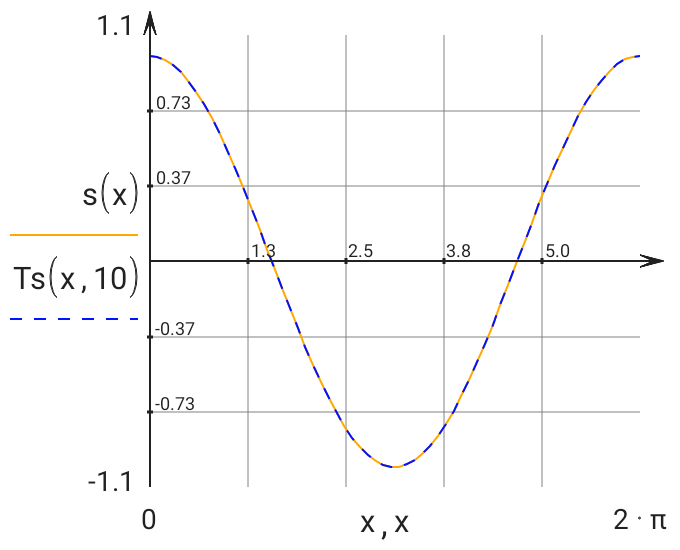
\includegraphics[width=0.45\textwidth]{graphics/series_and_integrals_fig1.png} \end{tabular}\end{center}

Sin embargo, hay un error numérico
debido al número limitado de términos
de aproximación N. La siguiente
función $\Delta$(x,N) describe este error:
\begin{center}\begin{tabular}{c}
  ${\Delta}(x,N) :=  \left| s \left( x\right)  - Ts \left( x,\, N\right)  \right| $
\end{tabular}\end{center}

Podemos graficar esta función en
coordenadas logarítmicas y ver que el
error numérico disminuirá si
introducimos más términos en la suma
de Taylor:
\begin{center}\begin{tabular}{c}
  $N := \left[ 3,\, 4 \,..\, 13 \right]$
\end{tabular}\end{center}
\begin{center}\begin{tabular}{c} 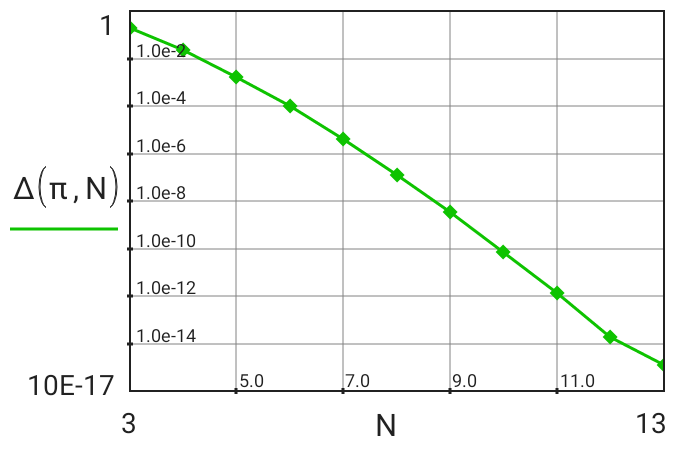
\includegraphics[width=0.45\textwidth]{graphics/series_and_integrals_fig2.png} \end{tabular}\end{center}

\subsection{Serie de binomios}

Consideremos esta función de poder:
\begin{center}\begin{tabular}{c}
  $f(x,{\alpha}) := {\left( 1 + x \right)}^{{\alpha}}$
\end{tabular}\end{center}

Esta función puede ser aproximada
usando serie de binomios:
\begin{center}\begin{tabular}{c}
  $Tf(x,{\alpha},N) := \displaystyle\sum_{n=0}^{N}  \left( \displaystyle\prod_{k=1}^{n} \frac{{\alpha} - k + 1}{k}\right)  \cdot {x}^{n}$
\end{tabular}\end{center}

También podemos graficar ambas
funciones (la función de potencia dada
y su aproximación) juntas en la misma
gráfica:
\begin{center}\begin{tabular}{c} 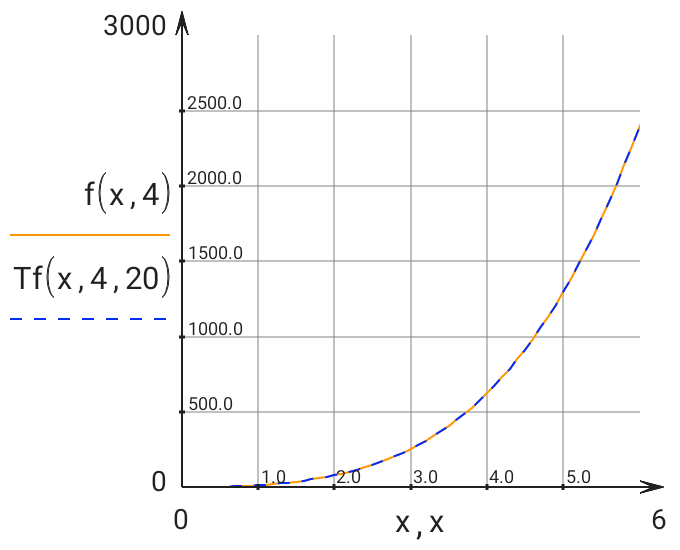
\includegraphics[width=0.45\textwidth]{graphics/series_and_integrals_fig3.png} \end{tabular}\end{center}

\subsection{Integrales}

También es posible calcular una
integral definida numéricamente usando
el método de Simpson. Por ejemplo,
podemos calcular la integral usando el
elemento ''Añadir vista de resultados'':
\begin{center}\begin{tabular}{c}
  $\displaystyle\int_{0}^{3 \cdot pi / 2}{cos \left( \frac{2 \cdot x}{9}\right) }^{-2}\, dx = 7.79423$
\end{tabular}\end{center}

La solución analítica es
\begin{center}\begin{tabular}{ccc}
  $I := \frac{9 \cdot \sqrt{3} }{2}$ &
  ,    &
  $I = 7.79423$ \cr
\end{tabular}\end{center}

El error numérico puede calcularse
como:
\begin{center}\begin{tabular}{c}
  $\displaystyle\int_{0}^{3 \cdot pi / 2}{cos \left( \frac{2 \cdot x}{9}\right) }^{-2}\, dx - I = 4.26681E-9$
\end{tabular}\end{center}

Este error depende del valor ''Cifras
significativas en el resultado'' que se
puede cambiar en el cuadro de diálogo
''Ajustes del documento'' disponible en
la barra de acciones:
\begin{center}\begin{tabular}{c} 
\includegraphics[width=0.45\textwidth]{graphics/series_and_integrals_fig4.png} \end{tabular}\end{center}

Si este valor aumenta, el umbral que
controla la precisión del método
Simpson también aumentará.